
\section{LAR wing Lift and Drag Models}

Low aspect ratio wings are wings where the ratio between the wing span and
the chord is small. Commertial aircrafts typically have high aspect ratio wings
to increase the amount of lift on the aircraft, but there are benefits of having
low aspect wings. Low aspect ratio aircrafts need to deal with less bending
stress because the wings are shorter. Also, the drag due to surface friction is
smaller because of the lower Reynold number because of the bigger lengthscale.
For paper airplanes, low aspect ratio wings are definitely better than high
aspect ratio wings because there is no way for paper to overcome the
bending stress.


\subsection{Previous Research}

A lot of research about the lift and drag  were done in the form of
micro-air vechicle research. This has the most relevance with paper airplanes because
micro-air vehicles operate on a Reynold number regime similar to paper airplanes. 
In 1999, Mueller showed that cambered plates offer better performance than flat plate wings, and
trailing-edge geometry does not have a strong effect on lift and drag
for thing wings at low Reynolds numbers. Also many experiments were done to experimentally
find the lift and drag coefficient of different wing shapes of different aspect ratios.

\subsection{Bollay Models}

The problem with the flat plate in the previous chapter is that it had to assume 
an aspect ratio of about zero in order to model it in that fasion. However, we can still
use the fact that the aspect ratio is small the model it in a different fashion.
Let us assume that the wing is thin and has a low aspect ratio. Let the angle of attack
 be $\alpha$. We can see that the normal component of the air
will have velocity. This is depicted in Figure~\ref{fig:bollay1}

\begin{figure}[hl]
  \centering
    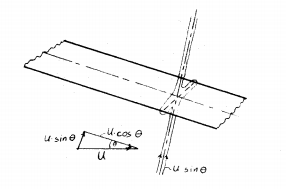
\includegraphics[scale=1]{figures/bollay1.png}
    \caption{normal component of air}
  \label{fig:bollay1}
\end{figure}


\[V\sin(\alpha)\]

If the angle is small enough this is approximately

\[V\alpha\]


It then follows that the lift force per unit length is just the normal velocity $V\alpha$ times the
rate of increase of a virtual additional mass. The virtual additional mass comes from the
added inertia from the fluid moving around the immersed object. For a thin line it is known
that.

\[dm=\frac{\pi}{4}\rho b^2 dx\]

If $\rho$ is the density of the fluid and $b$ and $x$ are the dimensions of the plate.

\[l = V\alpha \od{m}{t} = V^2\alpha \od{m}{x} \]

\[l = \pi \alpha \frac{\rho}{2}V^2 b \od{b}{x} \dif{x} \]

\[l = \pi \alpha \frac{\rho}{2} V^2 b \dif{b} \]

To get the entire lift force we can just integrate across the length of the chord. 
If the wings are rectangular than the result is:

\[L = \frac{\pi \alpha \rho V^2 b_{max}}{4} \]

This results in a lift coefficient $C_L$ of

\[ \frac{\pi}{2} \AR \alpha \].

Where $\AR$ is the aspect ratio.




